\chapterimage{arquitectos-tenerife.jpg}
\chapter{Despliegue}

\section{Introducción}

\newpage

\section{Diagrama de Sistemas}

Los diagramas de sistemas o paquetes son esquemas que ayudan a visualizar la forma de organización de una arquitectura. Además de ello permite visualizar la dependencia que hay en cada uno de los sistemas para así mejorar su estructura. Dentro de los diagramas de sistemas es posible encontrar dependencias lineales o cíclicas, el objetivo en la mayoría de casos es que la dependencia sea lineal, pues si la dependencia es cíclica significa que hay algo mal diseñado, y es allí donde el diseño por componentes hace su entrada para aliviar dicho problema. 
Para el caso particular del Sistema de Gestión de Monitorias se tiene el siguiente diagrama de sistemas:

\begin{figure}[H]
	\centering
	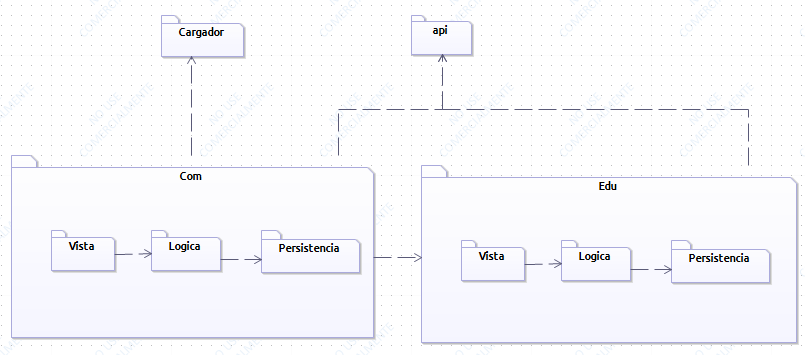
\includegraphics[width=1\linewidth]{dSistemas}
	\centering
	\caption{Diagrama de sistemas SGM}
	\label{fig:dSistemas}
\end{figure}

En el diagrama se aprecian dos grandes sistemas, Edu, el cuál abarca los subsistemas de Vista, Lógica y Persistencia correspondientes a cada componente y el cuál depende de un api. El otro sistema Com, también incluye los subsistemas de Edu, con la única diferencia de que este sistema es el aplicativo como tal, pues usa componentes, el cargador y un api.

\newpage

\section{Diagrama de Componentes}
\begin{figure}[H]
	\centering
	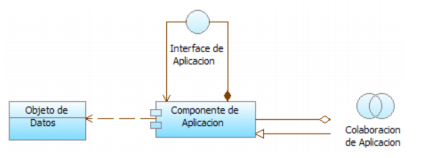
\includegraphics[width=0.7\linewidth]{componentes}
	\centering
	\caption{Estructura de un diagrama de componentes}
	\label{fig:componentes}
\end{figure}

El diagrama de componentes es similar a un diagrama de clases, pero da una visión más
general de la arquitectura del sistema. El diagrama de componentes muestra los componentes
del sistema, como un archivo de clases, un paquete, las bibliotecas compartidas, una base
de datos, etc., y cómo se relacionan entre sí. Los componentes individuales de un diagrama de
componentes se consideran en más detalle dentro de otros diagramas de UML, como los
diagramas de clases y los diagramas de casos de uso \cite{Kendall_2005}.

En el caso del sistema de Gestión de Monitoría, se planteó el diseño con 4 componentes básicos: El primero Clasificados, se encarga de gestionar la publicación y visualización de anuncios que los usuarios hagan en el sistema. El segundo componente, contactos gestiona las consultas de información de contacto de los participantes. El tercer componente, Monitorías, es el corazón del sistema, pues es allí donde se gestionan las horas y las certificaciones del aplicativo. Y por último el componente Perfil, gestiona toda la información del usuario, como su información personal y el número de horas que tienen los monitores.

\begin{figure}[H]
	\centering
	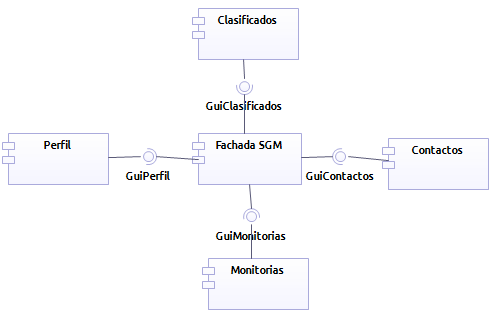
\includegraphics[width=0.7\linewidth]{dComponentes}
	\centering
	\caption{Diagrama de Componentes para el Sistema de Gestión de Monitorías}
	\label{fig:dcomponentes}
\end{figure}
\newpage


\section{Diagrama de Nodos}

\newpage


\section{Métricas}

